% document formatting
\documentclass[10pt]{article}
\usepackage[utf8]{inputenc}
\usepackage[left=1in,right=1in,top=1in,bottom=1in]{geometry}
\usepackage[T1]{fontenc}
\usepackage{xcolor}

% math symbols, etc.
\usepackage{amsmath, amsfonts, amssymb, amsthm}

% lists
\usepackage{enumerate}

% images
\usepackage{graphicx} % for images

% code blocks
\usepackage{minted, listings} 

% verbatim greek
\usepackage{alphabeta}

\graphicspath{{./assets/images}}

\newcommand{\solution}{\textbf{Solution:}} 
\newcommand{\example}{\textbf{Example: }}
\newcommand{\R}{\mathbb{R}}

\title{COM SCI 122 Week 6}

\author{Aidan Jan}
\date{\today}

\begin{document}
\maketitle

\section*{Clustering}

\subsection*{Central Dogma}
\begin{center}
    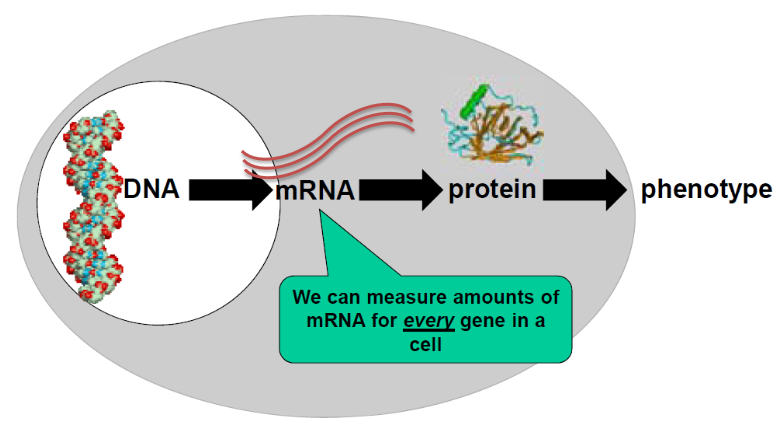
\includegraphics[scale=0.8]{W6_1.png}
\end{center}
\begin{itemize}
    \item DNA is transcribed to RNA, which is translated to protein.  Proteins determine phenotype.
    \item Phenotype is a lot easier to measure (e.g., gene expression) rather than genes themselves
\end{itemize}

\subsection*{Measuring Gene Expression}
\begin{itemize}
    \item Organisms typically have on the order of thousands or tens of thousands of protein coding genes (e.g., ~20000 genes in human)
    \item Gene expression profiling used to be limited to a single gene at a time.  This changed with the publication of the first microarray in 1995.
    \item By 1997, scaled up to measure expression of all yeast genes.
\end{itemize}
There are two additional major waves of technologies for measuring gene expression:
\begin{center}
    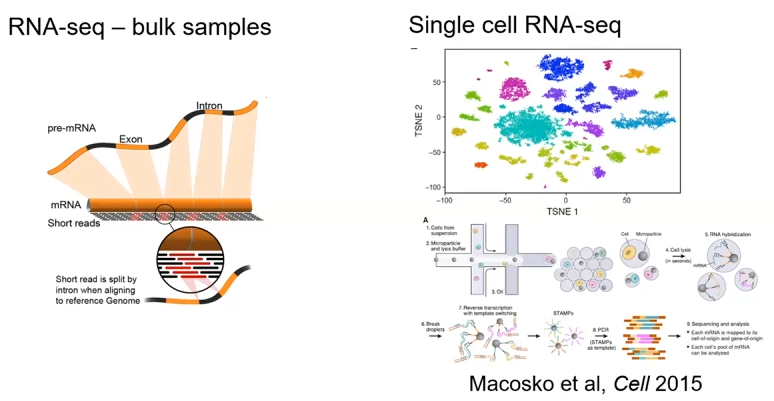
\includegraphics[width=0.8\textwidth]{W6_2.png}
\end{center}
Computational problem of clustering genes remains common accross technologies.

\subsection*{Gene Expression Data}
\begin{center}
    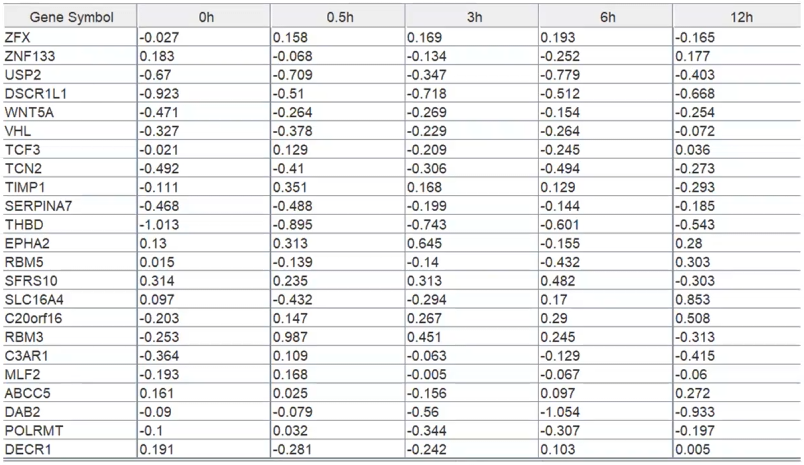
\includegraphics[width=\textwidth]{W6_3.png}
\end{center}
\begin{itemize}
    \item Each row is a gene.
    \item Each column is a different experimental condition
\end{itemize}

\subsection*{Heatmap Representation of Gene Expression Data}
\begin{center}
    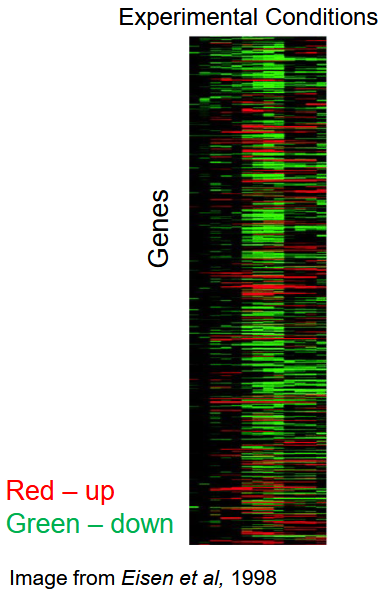
\includegraphics[scale=0.6]{W6_4.png}
\end{center}

\subsection*{Gene Expression Clustering Problem}
\begin{itemize}
    \item Group unlabeled data points
    \item Informally want:
    \begin{itemize}
        \item Data points "near" each other in the same clusters
        \item Data points "far" from each other in different clusters
    \end{itemize}
\end{itemize}
\begin{center}
    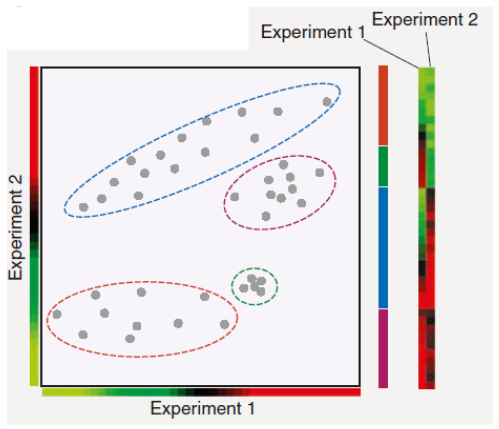
\includegraphics[scale=0.6]{W6_5.png}
\end{center}
Why do we cluster genes by expression?
\begin{itemize}
    \item Genes with similar gene expression patterns across experimental conditions are often involved in the same biological process or co-regulated (e.g., regulated by the same transcription factor)
    \item By identifying sets of genes with similar expression patterns can lead to insight into biological processes associated with the conditions, gene regulatory mechanism, and roles of genes with unknown function
    \begin{itemize}
        \item Example: identify sequence patterns around transcription start sites of genes with similar expression patterns (ch. 2)
    \end{itemize}
\end{itemize}

\section*{Clustering Algorithms}
\begin{itemize}
    \item Many clustering algorithms exist.  E.g., Hierarchical clustering, K-means clustering
\end{itemize}
\begin{center}
    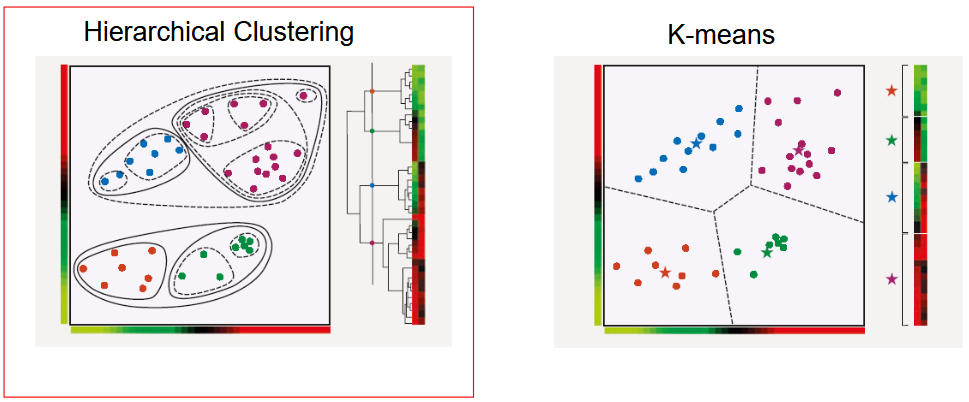
\includegraphics[width=\textwidth]{W6_6.png}
\end{center}

\section*{Hierarchical Clustering}
\begin{enumerate}
    \item Initially each point is its own cluster.
    \item Find the pair of clusters with the smallest distance between them or equivalently are the most similar.
    \item Merge into parent cluster.
    \item Repeat steps 2 and 3 until the desired number of clusters remain.
\end{enumerate}

\subsubsection*{How do we measure distance?}
\begin{center}
    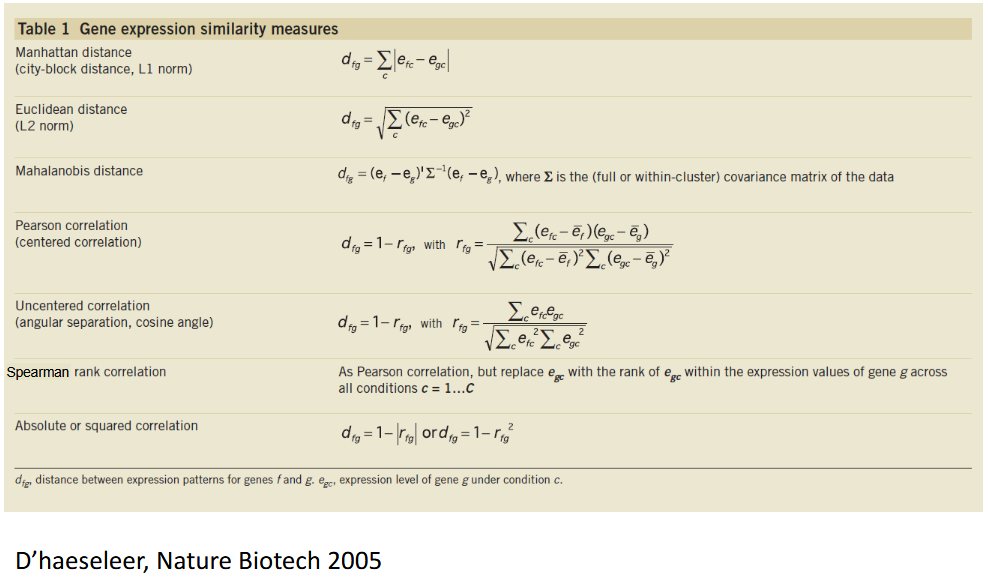
\includegraphics[width=\textwidth]{W6_7.png}
\end{center}
\begin{itemize}
    \item Pearson Correlation is popular since it clusters based on shape and relative changes which can often be more informative than absolute expression levels.
    \begin{itemize}
        \item However, the Pearson correlation can fail to provide output if the variance is 0.  In this case, it is undefined.
        \item Typically, filter genes do not change expression before clustering.
    \end{itemize}
\end{itemize}

\subsubsection*{Measuring Distance between Clusters}
\begin{itemize}
    \item Single Linkage Clustering:
    \[D(X, Y) = \text{min}_{x \in X, y \in Y} d(x, y)\]
    \item Complete Linkage Clustering:
    \[D(X, Y) = \text{max}_{x \in X, y \in Y} d(x, y)\]
    \item Average Linkage Clustering:
    \[D(X, Y) = \frac{1}{|X| \cdot |Y|} \sum_{x \in X} \sum_{y \in Y} d(x, y)\]
    \item Centroid Linkage Clustering:
    \[D(X, Y) = \Vert c_X - c_Y\Vert\]
    \begin{itemize}
        \item where $c_X$ and $c_Y$ are the mean of $X$ and $Y$ and data assumed to be in $\mathbb{R}^d$
    \end{itemize}
\end{itemize}
\begin{center}
    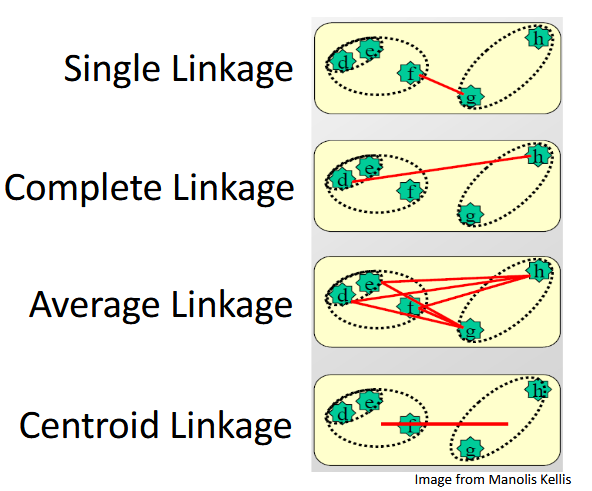
\includegraphics[scale=0.6]{W6_8.png}
\end{center}

\subsubsection*{Hierarchical Clustering Example 1}
\begin{center}
    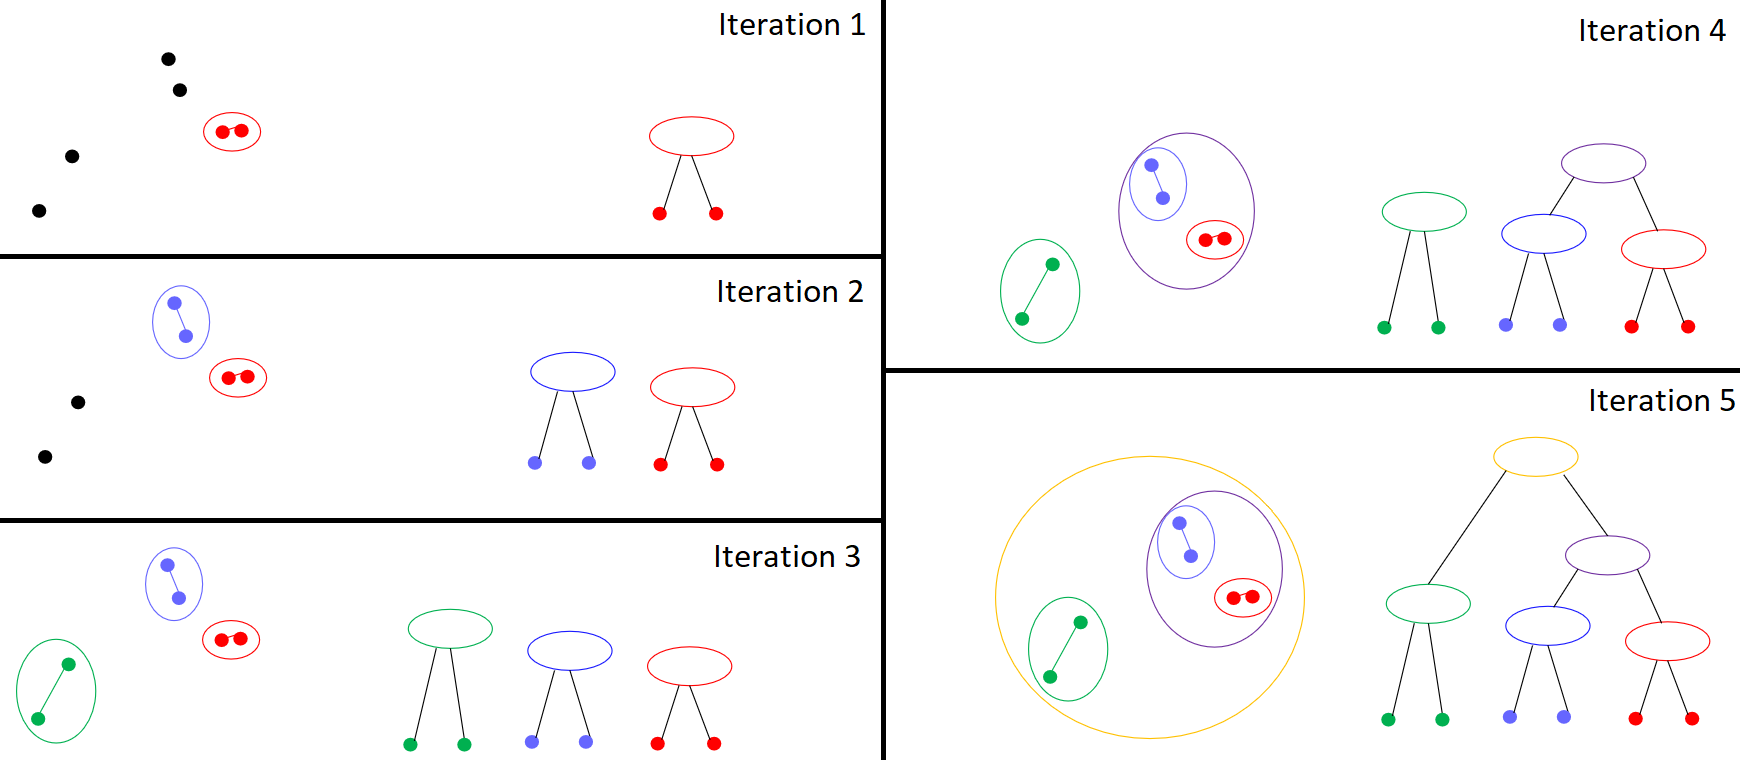
\includegraphics[width=\textwidth]{W6_9.png}
\end{center}

\subsubsection*{Hierarchical Clustering Example 2}
Suppose we want to perform hierarchical clustering with Euclidean distance using single linkage clustering to the four data points below.
\begin{center}
    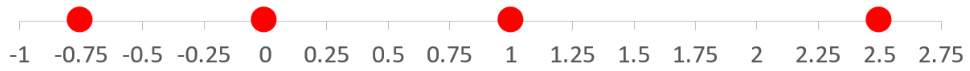
\includegraphics[width=\textwidth]{W6_10.png}
\end{center}
Finding the distance between each pair of points, the left two points are the closest together.  Therefore, we merge them into one group.
\begin{center}
    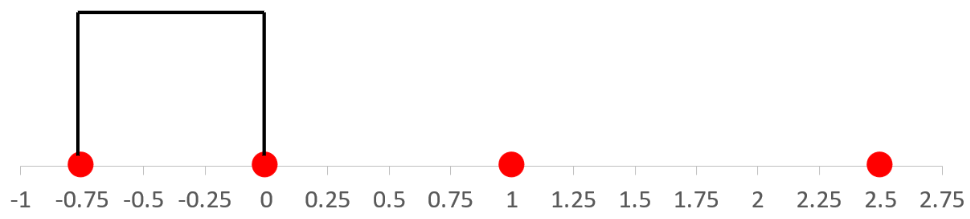
\includegraphics[width=\textwidth]{W6_11.png}
\end{center}
The next closest group would be merging the (1) into the group we just created, since the distance between the (1) point is 1, and the distance between (1) and (2.5) is 1.5.
\begin{center}
    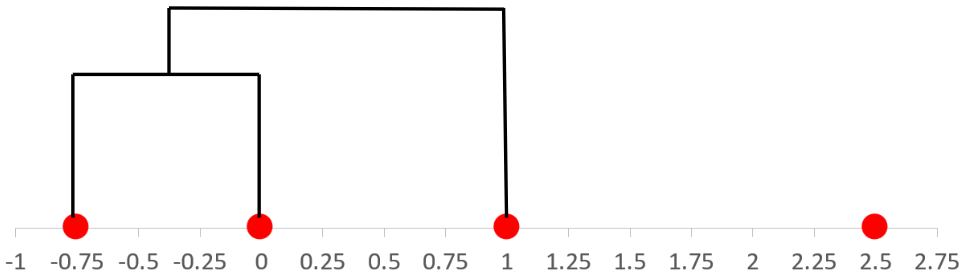
\includegraphics[width=\textwidth]{W6_12.png}
\end{center}
Finally, we merge the 2.5 point.
\begin{center}
    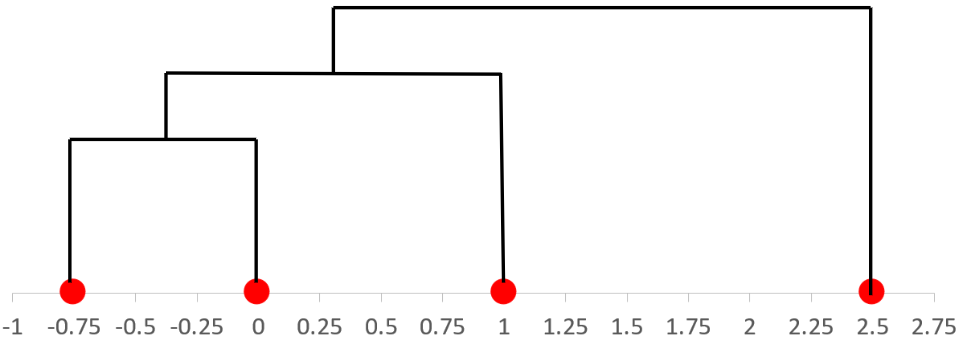
\includegraphics[width=\textwidth]{W6_13.png}
\end{center}

\subsubsection*{Hierarchical Clustering Example 3}
Suppose we want to perform hierarchical clustering with the same points as above, but this time, we use \textbf{complete linkage clustering}.
\begin{center}
    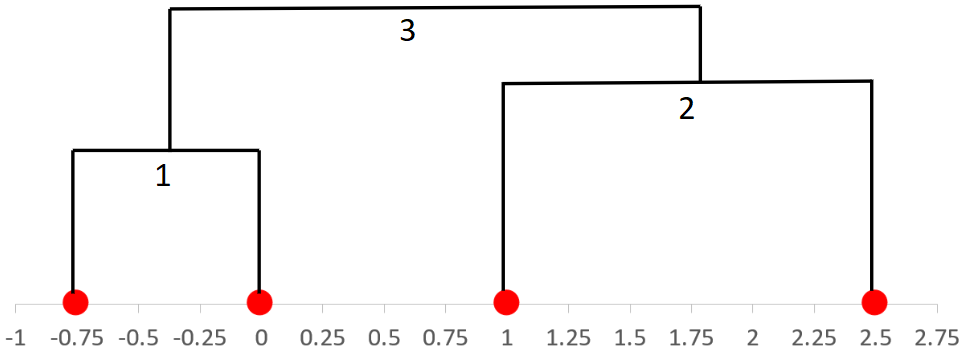
\includegraphics[width=\textwidth]{W6_14.png}
\end{center}
\begin{itemize}
    \item Notice that complete linkage clustering led to a different dendogram than single linkage.
\end{itemize}

\subsubsection*{Hierarchical Clustering Example 4}
Same points, but this time with average linkage clustering.
\begin{center}
    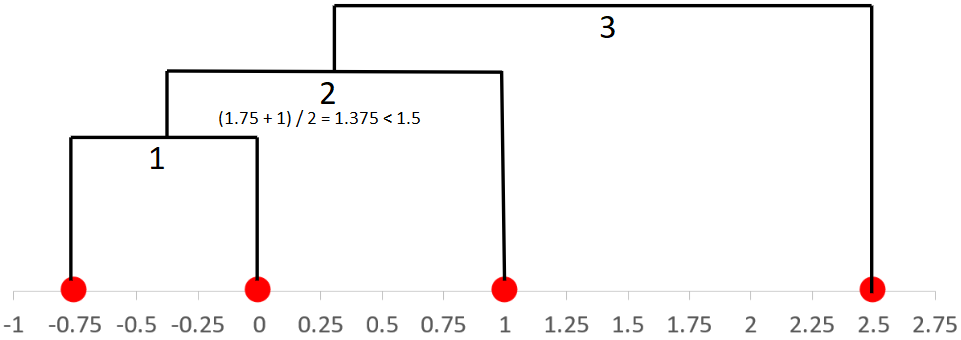
\includegraphics[width=\textwidth]{W6_15.png}
\end{center}

\subsection*{Runtime Complexity of Hierarchical Clustering}
\begin{itemize}
    \item Let $n$ be the number of data points
    \item O($n^2$) time to compute all pairwise distances
    \item O($n$) iterations
    \item O($n^3$) if all pairwise distances recomputed and/or iterated over each iteration
    \item Depending on details of linkage method and implementation, this can run in O($n^2$) or O($n^2 \log n$) time
\end{itemize}

\subsection*{Ordering Leaves}
Often more visual focus goes to the heatmap and the row ordering than the dendogram.  
\begin{center}
    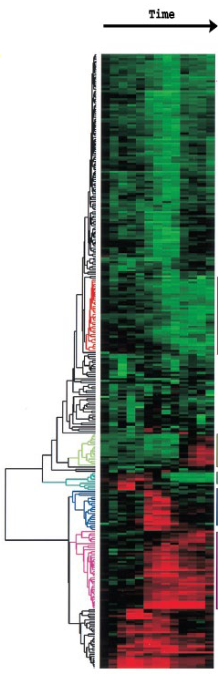
\includegraphics[scale=0.5]{W6_16.png}
\end{center}
\textbf{Question:} Does hierarchical clustering uniquely determine an ordering of leaves (rows)?
\begin{itemize}
    \item No!  Two leaves can be swapped around without changing the structure of the hierarchical clustering.
    \item The two structures below have the same hierarchical clustering, but different orders.
\end{itemize}
\begin{center}
    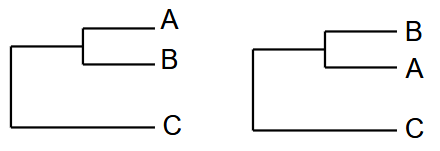
\includegraphics[scale=0.8]{W6_17.png}
\end{center}
\textbf{Question:} How many possible orderings are there for a hierarchical clustering of $n$ data points?
\begin{itemize}
    \item $2^{n - 1}$.  This is because the hierarchical clustering always produces a binary tree.  If there are $n$ leaves, then there are $2^{n - 1}$ internal nodes.
    \item Each internal node can be flipped.
\end{itemize}
\textbf{Question:} How should we select among possible orderings?
\begin{itemize}
    \item Idea: pick an ordering that minimizes distance between adjacent leaves or equivalently maximizes similarity.
\end{itemize}

\subsection*{Optimal Ordering Leaves}
\textbf{Problem:} Order leaves of hierarchical clustering dendrogram to minimize sum of distances between neighboring leaves or equivalently maximize similarity of neighboring leaves.\\\\
From Eisen et al, 1998 paper:\\
\fbox{
    \parbox{\textwidth}{
        \textbf{Ordering of Data Tables.}  For any dendrogram of $n$ elements, there are $2^{n - 1}$ linear orderings consistent with the structure of the tree (at each node, either of the two elements joined by the node can be ordered ahead of the other).  An optimal linear ordering, one that maximizes the similarity of adjacent elements in the ordering, is impractical to compute.
    }
}
\begin{itemize}
    \item It turns out that solving this problem with brute force will take expoenntial time.  However, it is possible to compute this in polynomial time - O($n^3$).
\end{itemize}

\subsection*{Optimal Ordering Leaves in O($n^3$) time}
\begin{itemize}
    \item T($v$) - subtree rooted at $v$
    \item M($v, i, j$) - cost of optimal tree rooted at $v$ with start and end leaves $i$ and $j$ respectively where $i, j$ are leaves in T($v$)
    \item M($v, v, v$) = 0
    \item $\text{M}(v, i, j) = \min_{x \in \text{T}(u), y \in \text{T}(w)} \text{M}(u, i, x) + \text{d}(x, y) + \text{M}(w, y, j)$
    \begin{itemize}
        \item $u$ is the left sub-child
        \item $w$ is the right sub-child
    \end{itemize}
    \item Dynamic programming!
\end{itemize}
\begin{center}
    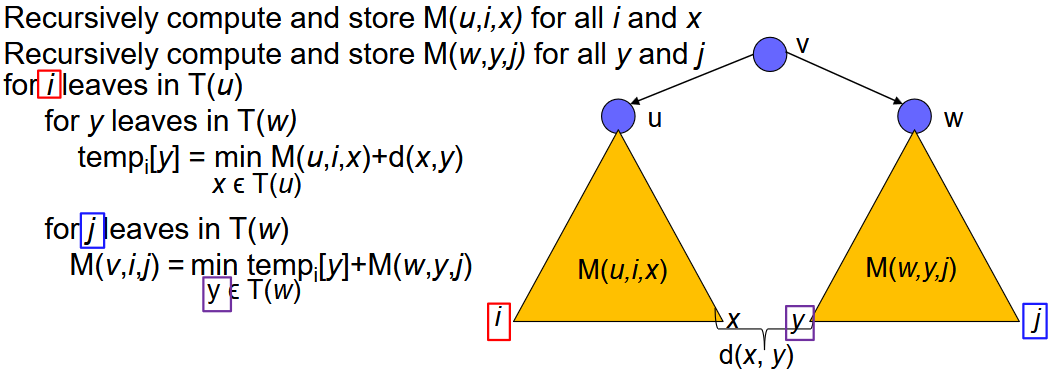
\includegraphics[width=\textwidth]{W6_18.png}
\end{center}
\subsubsection*{Proof of O($n^3$) time}
\begin{itemize}
    \item Let $F(n)$ be the total time to compute $M(v, i, j)$ for all $i, j$ in a tree with $n$ leaves.
    \item Let $r$ be the number of leaves in subtree $T(u)$
    \item Let $s$ be the number of leaves in subtree $T(w)$
    \[F(n) = F(r) + F(s) + O(r^2s) + O(rs^2)\]
    \item We have $r + s = n$ and
    \[(r^3 + s^3 + r^2s + rs^2) \leq (r + 3)^3 = n^3\]
    \item By induction it follows that $F(n)$ is O($n^3$)
\end{itemize}

\subsection*{Ordering Leaves Optimally}
\begin{center}
    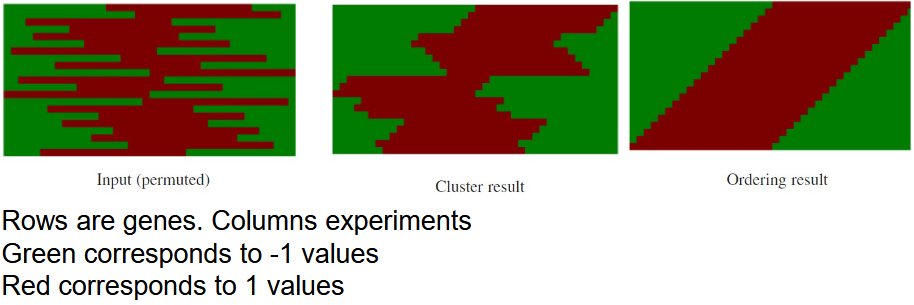
\includegraphics[width=\textwidth]{W6_19.png}
\end{center}

\subsection*{Getting Clusters from Hierarchical Clustering}
How can we get $k$ clusters from hierarchical clustering?
\begin{center}
    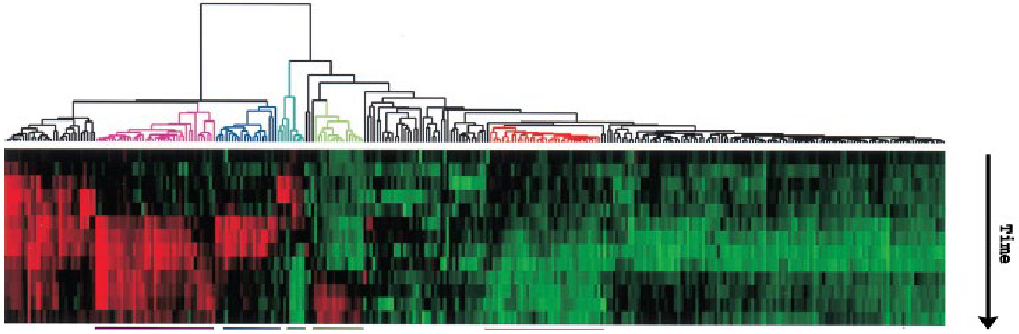
\includegraphics[width=\textwidth]{W6_20.png}
\end{center}
\begin{itemize}
    \item Idea: cut tree to undo last $k - 1$ merges.
\end{itemize}
\begin{center}
    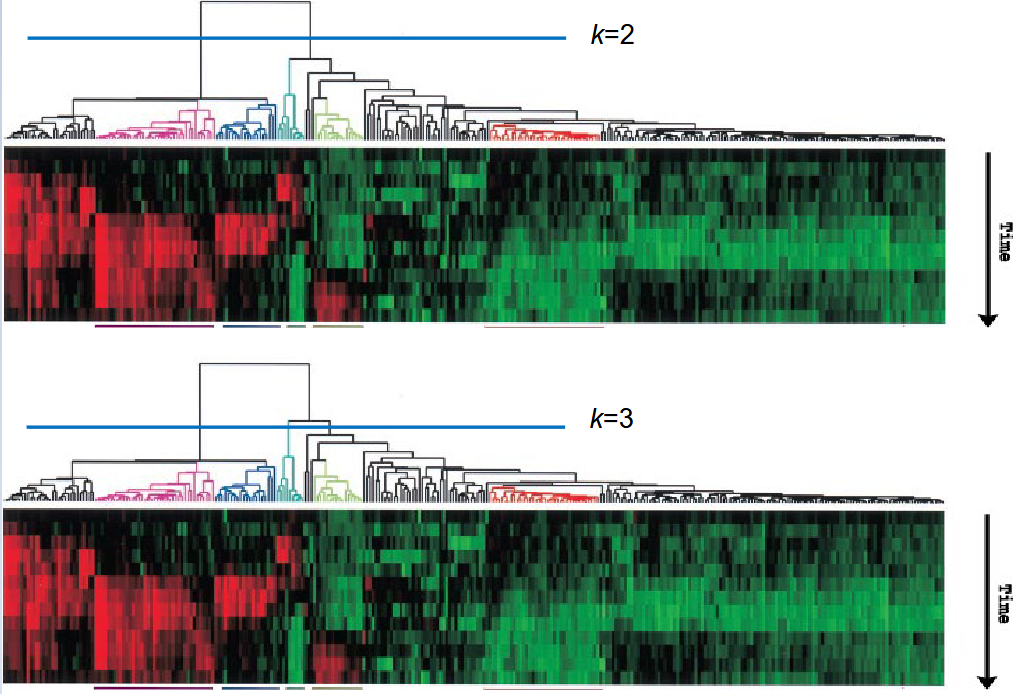
\includegraphics[width=\textwidth]{W6_21.png}
\end{center}
\begin{itemize}
    \item This method is popular since it shows all the data in a hierarchy, but limited theoretical basis for resulting clusters
    \begin{itemize}
        \item (i.e., no associated optimization criteria or statistical model)
    \end{itemize}
\end{itemize}

\section*{K-means Clustering}
\subsection*{The K-means Objective Function}
\[\text{argmin} \sum_{i = 1}^k \sum_{x_j \in S_i} \Vert x_j - \mu_i \Vert^2\]
\begin{itemize}
    \item $\mu_i$ = Mean of cluster $i$
    \item $S_i$ = Data points assigned to cluster $i$
\end{itemize}
Can be motivated by minimizing loss of information in compression
\begin{itemize}
    \item an encoder function: $\text{ENCODE} \::\: \mathfrak{R}^d \rightarrow [1 \dots k]$
    \item a decoder function: $\text{DECODE} \::\: [1 \dots k] \rightarrow \mathfrak{R}^d$
    \item We define distortion to be
    \[\text{Distortion} = \sum_{i = 1}^n(x_i - \text{DECODE}[\text{ENCODE}(x_i)])^2\]
\end{itemize}
After initializing clustering centers, iterate between two steps:
\begin{itemize}
    \item Re-assign data points to its closest cluster mean
    \item Recompute the cluster mean of the points assigned to each cluster
\end{itemize}

\subsubsection*{K-means Algorithm Example}
\begin{enumerate}
    \item Ask user how many clusters they'd like.
    \begin{itemize}
        \item E.g., $k = 5$
    \end{itemize}
    \item Randomly guess $k$ cluster center locations
    \begin{center}
        \includegraphics*[scale=0.5]{W6_22.png}
    \end{center}
    \begin{itemize}
        \item Above: blue dots are data points, red dots are randomly guessed centers.
    \end{itemize}
    \item Each datapoint finds out which center it's closest to.  (Thus, each center "owns" a set of datapoints)
    \begin{center}
        \includegraphics*[scale=0.5]{W6_23.png}
    \end{center}
    \item Each center finds the centroid of the points it owns, and moves there.
    \begin{center}
        \includegraphics*[scale=0.5]{W6_24.png}
    \end{center}
    \item Repeat 3-4 until the centers no longer move, or the program is terminated.
\end{enumerate}

\subsection*{K-means Convergence}
Is the k-means algorithm guaranteed to converge (i.e., no change in objective cost)?
\begin{itemize}
    \item \textbf{Yes.}  The algorithm will converge since there are only a finite number of ways of partitioning the set of data points into k-groups.  Each iteration would need to visit a new configuration since it cannot increase objective value being minimized between iterations.
\end{itemize}
Going back to the objective function, to prove convergence, we need to claim that neither step (out of reassigning data points and moving center) would increase the objective function.\\\\
For the reassign step:
\begin{itemize}
    \item For each point $x_j \in S_i$, either
    \begin{itemize}
        \item it is closer to its current center $i \rightarrow$ no change
        \item it is closer to another center $m \rightarrow$ objective function improves since $\Vert x_j - \mu_m \Vert^2 < \Vert x_j - \mu_i \Vert^2$
    \end{itemize}
\end{itemize}
For the recompute cluster mean step:
\begin{itemize}
    \item To find the minimum, take partial derivatives and set them equal to 0.
    \[\frac{\partial}{\partial \mu_{i, d}} \sum_{i = 1}^k \sum_{x_j \in S_i} \Vert x_j - \mu_i \Vert^2 = \frac{\partial}{\partial \mu_{i, d}} \sum_{x_j \in S_i} \Vert x_j - \mu_i \Vert^2 = -2 \sum_{x_j \in S_i} (x_{j, d} - \mu_{i, d})\]
    \item The above is 0 when $\mu_{i, d} = \frac{\sum_{x_j \in S_i} (x_{j, d})}{|S_i|}$ (i.e., cluster center)
\end{itemize}

\subsection*{K-means Optimal Solution}
Is the k-means algorithm guaranteed to find an optimal solution?
\begin{itemize}
    \item \textbf{No.}  Consider if the clusters were initiallized like below:
\end{itemize}
\begin{center}
    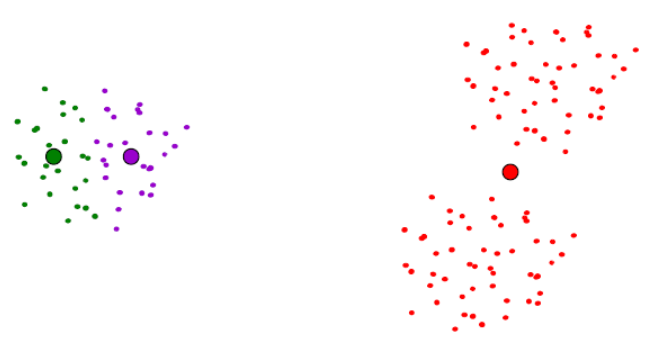
\includegraphics[width=\textwidth]{W6_25.png}
\end{center}
Is there a better way to initialize clusters, so this doesn't happen?

\subsection*{One Idea - Furthest Point Heuristic}
\begin{itemize}
    \item Pick the first cluster center to be one arbitrarily selected point
    \item Iteratively pick cluster centers to be remaining points that are furthest from any selected point
\end{itemize}
\begin{center}
    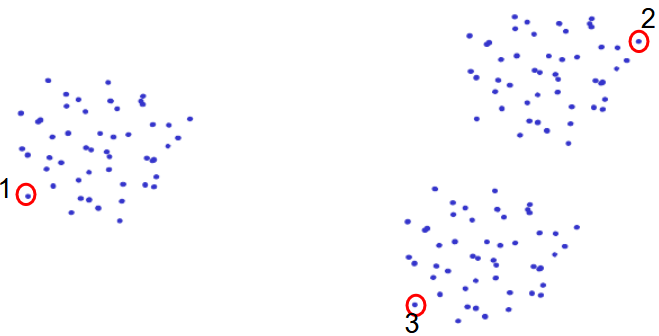
\includegraphics[width=\textwidth]{W6_26.png}
\end{center}
Approximation algorithm to k-centers problem - minimize maximum distance of any point to its closest center\\\\
\textbf{Question:} Can this fail to lead to a good clustering?
\begin{itemize}
    \item \textbf{Yes} - suppose there are two very far out points:
\end{itemize}
\begin{center}
    \includegraphics*[width=\textwidth]{W6_27.png}
\end{center}
\textbf{Question:} Any ideas for initializing the centers that would spread the points while being less sensitive to outliers?
\begin{itemize}
    \item Pick first cluster center to be one arbitrarily selected point
    \item Iteratively select a cluster center $x'$ to be a point in the data probabilistically, where the probabilities are determined by
    \[\frac{D(x')^2}{\sum_{x \in X} D(x)^2}\]
    \begin{itemize}
        \item where $D(x)$ is the distance of $x$ to its closest currently selected cluster center and $X$ is the set of all points
    \end{itemize}
\end{itemize}

\subsection*{Run-time of k-means algorithm}
\begin{itemize}
    \item Let $n$ be the number of data points
    \item Let $d$ be the number of dimensions in the data
    \item Let $k$ be the number of clusters
    \item Let $i$ be the number of iterations
    \item The run-time of the k-means algorithm is O($ndki$)
    \item In the worst case, the number of iterations is O($2^{\Omega(\sqrt{n})}$)
    \item in practice, we will need fewer iterations and can terminate early based on a fixed number of iterations or small changes to objective.
\end{itemize}

\section*{More Clustering Algorithms}
\subsection*{Gaussian Mixture Models and the EM Algorithm}
What are some potential limitations in the assumptions behind k-means clustering?
\begin{itemize}
    \item It assumes we can be completely confident in the cluster assignment of each data point (i.e., makes "hard assignments" of points to clusters)
    \item There could be cluster shapes not captured based on partitioning the space based on the distance to the nearest cluster
\end{itemize}
\begin{center}
    \includegraphics*[width=\textwidth]{W6_28.png}
\end{center}
\subsubsection*{Motivating Example:}
\begin{itemize}
    \item Suppose in a response to a biological stimulus we have three groups of genes: activated, unaffected, and repressed
    \item Further, suppose within each group we know the gene expression follows a gaussian (normal) distribution with variance 1, and means -1.5, 0, 1.5 for the repressed, unaffected, and activated groups, respectively.
    \item Also assume a priori a gene is equally likely to be in any one of the three groups.
\end{itemize}
\begin{center}
    \includegraphics*[width=\textwidth]{W6_29.png}
\end{center}
Suppose we simulate the expression values for 20 genes from each group based on the assumptions and observe the following set of values:
\begin{center}
    \includegraphics*[width=\textwidth]{W6_30.png}
\end{center}
\textbf{Question:} Is there necessarily a partitioning into three intervals such that all points in each interval belong to the same group?   (No.)
\begin{itemize}
    \item We can't always assume each point's true group corresponds to its closest center.
    \item What can we do?  Use \textbf{probabilistic soft assignments}
\end{itemize}
\subsubsection*{Problem}
Suppose we were given a set of unlabeled points such as above.  We are willing to assume each point was generated by one of $K$ gaussian distributions.  Each of the $K$ gaussian distributions has a prior probability associated with it.\\\\
We would like to be able to:
\begin{enumerate}
    \item Find a set of $K$ gaussian distributions and corresponding priors that "best describe" the data
    \item Give "soft" probabilistic cluster assignments to each point based on the $K$ gaussian distributions and corresponding priors that "best describe" the data
\end{enumerate}
We will first consider a simpler version of (2) where we will compute “soft" probabilistic cluster assignment when given K gaussian distributions and corresponding priors

\subsection*{Estimating Assignment Probabilities}
\begin{itemize}
    \item Referring to the above graph, what is the probability that a gene with the expression value of -1 is in the unaffected group?
\end{itemize}
\begin{center}
    \includegraphics*[scale=0.7]{W6_31.png}
\end{center}
\[\frac{0.242}{0.352 + 0.242 + 0.018} = \boxed{0.395 \text{ unaffected group}}\]
If we do the same math, we can find the probability that it is in the activated group (0.029) and the probability that it is in the repressed group (0.575).\\\\
Now, suppose we instead assume that the prior probability a gene is in the unaffected group is \textbf{0.5} and \textbf{0.25} for both the repressed and activated groups.  (Instead of all 1-to-1.)
\begin{center}
    \includegraphics*[scale=0.7]{W6_32.png}
\end{center}
Now, the chance that it is in the \textbf{repressed} group is:
\[\frac{0.25 \times 0.352}{0.25 \times 0.352 + 0.5 \times 0.242 + 0.25 \times 0.018} = 0.412\]
\begin{itemize}
    \item In general, we can estimate cluster assignment probability for cluster $k$ of data point $x$ as
    \[\frac{\pi_k f(x | \mu_k, \sigma_k^2)}{\sum_{i = 1}^K \pi_i f(x|\mu_i, \sigma_i^2)}\]
    \begin{itemize}
        \item where $\pi_i$ is the cluster prior and $f$ is a gaussian density with mean $\mu$ and variance of $\sigma^2$.
    \end{itemize}
    \item If we know the parameters of the gaussians and cluster priors, it is easy to compute cluster assignment probabilities.
\end{itemize}
We will now go back to the problem - instead, we will consider a simpler version of (1) where we compute $K$ gaussian distributions and corresponding priors when we know the "soft" probabilistic cluster assignment of each data point.

\subsection*{Estimating Gaussian Means}
Suppose we do not know the means of the gaussians.  First consider the case we are given hard assignments to clusters indicated with a one-hot encoding.
\begin{center}
    \includegraphics*[width=0.8\textwidth]{W6_33.png}
\end{center}
What should the estimated mean of cluster 1 be?
\[\frac{-2 - 1.5}{2} = -1.75 \text{ (cluster 1)}\]
We can estimate the cluster 2 and 3 means as well.
\[\frac{0 + 0.25 + 0.5}{3} = 0.25 \text{ (cluster 2)}\]
\[\frac{2 + 3}{2} = 2.5 \text{ (cluster 3)}\]
Now, consider if we do not know the means of the gaussians but are given soft assignments to clusters with the indicated probabilities
\begin{center}
    \includegraphics*[width=0.8\textwidth]{W6_34.png}
\end{center}
Now, we can estimate the means by:
\begin{align*}
    \frac{-2 \times 0.87 + -1.5 \times 0.75 + 0 \times 0.20 + 0.25 \times 0.13 + 0.5 \times 0.08 + 2 \times 0 + 3 \times 0}{0.87 + 0.75 + 0.20 + 0.13 + 0.08 + 0 + 0} &= -1.38 \text{ cluster 1}\\
    \frac{-2 \times 0.13 + -1.5 \times 0.24 + 0 \times 0.61 + 0.25 \times 0.59 + 0.5 \times 0.54 + 2 \times 0.13 + 3 \times 0.03}{0.87 + 0.75 + 0.20 + 0.13 + 0.08 + 0 + 0} &= 0.06 \text{ cluster 2}\\
    \frac{-2 \times 0 + -1.5 \times 0.01 + 0 \times 0.20 + 0.25 \times 0.28 + 0.5 \times 0.37 + 2 \times 0.87 + 3 \times 0.97}{0.87 + 0.75 + 0.20 + 0.13 + 0.08 + 0 + 0} &= 1.81 \text{ cluster 3}
\end{align*}

\subsection*{Estimating Gaussian Priors}
Now, we can estimate the priors:
\begin{align*}
    \frac{(0.87 + 0.75 + 0.20 + 0.13 + 0.08 + 0 + 0)}{7} &= 0.29\\
    \frac{(0.13 + 0.24 + 0.61 + 0.59 + 0.54 + 0.13 + 0.03)}{7} &= 0.32\\
    \frac{(0 + 0.01 + 0.2 + 0.28 + 0.37 + 0.87 0.97)}{7} &= 0.39
\end{align*}

\subsection*{Estimating Parameters in General Given Assignment Probabilities}
The mean estimate for cluster $i$:
\[\mu_i = \frac{\sum_{j = 1}^N w_{ij} x_j}{\sum_{j = 1^N w_{ij}}}\]
where 
\begin{itemize}
    \item $w_{ij}$ is the "soft" assignment probability for data point $x_j$ to cluster $i$
    \item $N$ is the number of data points
\end{itemize}
The cluster prior estimate for cluster $i$ when estimating from data:
\[\pi_i = \frac{\sum_{j = 1}^N w_{ij}}{N}\]
Variance prior estimate for cluster $i$ when assuming different unknown variances:
\[\sigma_i^2 = \frac{\sum_{j = 1}^N w_{ij} (x_j - \mu_i)^2}{\sum_{j = 1}^N w_{ij}}\]
Note that $\mu_i$ is the re-estimated value from the current iteration.

\subsection*{The Expectation-Maximization (EM) Algorithm}
\begin{itemize}
    \item Initialize parameters of model
    \item Iterate between these two steps until a stopping criteria is met (e.g., minimum change of likelihood, number of iterations)
    \begin{itemize}
        \item Expectation (E)-step: Compute cluster assignment probabilities of each data point given model parameters
        \item Maximization (M)-step: Recompute the model parameters based on the soft cluster assignment probabilities
    \end{itemize}
    \item We have already seen how to compute the E and M steps separately
    \item This is also analogous to the k-means algorithm but with soft assignments instead of hard assignments
    \begin{itemize}
        \item E-step - soft version of recomputing cluster assignments
        \item M-step - soft version of recomputing cluster parameters
    \end{itemize}
\end{itemize}

\subsection*{Random Initialization}
(E-Step) We will assume uniform cluster priors and variance of 1 is known and only mean is being estimated.
\begin{center}
    \includegraphics*[width=\textwidth]{W6_35.png}
\end{center}
(M-Step) We will now re-estimate based on weighted average with weights determined by cluster assignment probabilities
\begin{center}
    \includegraphics*[width=\textwidth]{W6_36.png}
\end{center}
\subsection*{Optimization Objective}
Log-likelihood of data given model assumptions:
\[\text{max} \sum_{j = 1}^N \log \sum_{i = 1}^K \pi_i f(x_j|\mu_i, \sigma_i^2)\]
\begin{itemize}
    \item $f$ is the normal density
    \item $\pi_i$ is the cluster prior and values add up to 1
    \item $N$ is the number of data points
    \item $K$ is a hyper-parameter on the number of clusters
    \item Optimization is over values of $\mu_i$, $\sigma_i^2$, $\pi_i$ not considered fixed.
\end{itemize}
EM algorithm is a way to try to optimize the function by introducing a latent variable $z_j$ of the assignment of each data point to a cluster
\[\text{max} \sum_{j = 1}^N \log \sum_{i = 1}^K f(x_j | \mu_i, \sigma_i^2, z_j = i) p(z_j = i | \pi_i)\]
\begin{itemize}
    \item The second term ($p(z_j = i | \pi_i)$) is the probability that $z_j$ is in class $i$
    \item Latent variables are estimated probabilistically through the expectation step.
    \item Each iteration is non-decreasing.  No guarantee of global maximum.
\end{itemize}

Using the EM algorithm solves one of the problems we had in K-means clustering - which was there could be cluster shapes not captured based on partitioning the space based on the distance to the nearest cluster.

\subsection*{Generalizing to Multiple Dimensions}
Approach generalizes to multivariate gaussian distributions:
\[f_X(x_1, \dots, x_k) = \frac{\exp\left(-\frac{1}{2}(x - \mu)^T \Sigma^{-1}(x - \mu)\right)}{\sqrt{(2\pi)^k |\Sigma|}}\]
In this case, $\Sigma$ represents the covariance matrix.\\\\
In the two-dimensional case, we have:
\[\mu = \begin{pmatrix} \mu_X \\ \mu_Y \end{pmatrix}, \hspace{1cm} \Sigma = \begin{pmatrix} \sigma_X^2 & \rho \sigma_X \sigma_Y \\ \rho \sigma_X \sigma_Y & \sigma_Y^2 \end{pmatrix}\]
where $\rho$ is the Pearson correlation coefficient

\subsubsection*{Example of Different Bivariate Gaussian Distributions}
\begin{center}
    \includegraphics*[scale=0.8]{W6_37.png}
\end{center}

\subsection*{Example of EM Algorithm in Multiple Dimensions}
\begin{center}
    \includegraphics*[scale=0.8]{W6_38.png}
\end{center}

\subsection*{Multivariate Gaussians Do Not Capture All Shapes}
Multivariate gaussians only capture spherical and oval shapes.  Here is an example of data not expected to be well captured by multivariate gaussian distributions:
\begin{center}
    \includegraphics*[scale=0.9]{W6_39.png}
\end{center}

\section*{Clustering Short Time-Series Data}
\begin{itemize}
    \item Biological processes occur over time (e.g., stress response, immune response, development) and frequently studied with gene expression experiments
    \item Most time series gene expression data sets are short (3-8 time points)
    \begin{center}
        \includegraphics*[width=\textwidth]{W6_40.png}
    \end{center}
    \item Genes with similar expression patterns over time are often involved in the same biological process or are co-regulated
\end{itemize}

\subsection*{Limitations of Standard Clustering Methods for Time Series Data}
\begin{itemize}
    \item Having few time points can pose a challenge for traditional time
    series models (e.g. autoregressive equations) 
    \item Commonly used methods such as k-means and hierarchical clustering do not use the temporal ordering of experiments
    \item Thousands of genes and few time points many patterns by random chance
    \begin{itemize}
        \item Standard clustering methods do not differentiate between real and random patterns
    \end{itemize}
    \begin{center}
        \includegraphics*[width=\textwidth]{W6_41.png}
    \end{center}
    The above image are clusters from K-means on simulated noise (all values drawn independently from the identical distribution)
\end{itemize}

\subsection*{Method Overview}
Approach: Determine temporal patterns with significantly more genes than expected compared to a random ordering of time\\\\
Steps:
\begin{enumerate}
    \item Define temporal profiles independent of data
    \item Assign genes to most closely matching profile
    \item Compute expected number of genes per profile
    \item Determine statistically significant profiles
\end{enumerate}

\subsubsection*{Step 1}
Define a set of distinct and representative model temporal profiles \textbf{independent} of the data.
\begin{center}
    \includegraphics*[width=\textwidth]{W6_42.png}
\end{center}
Start with all temporal profile shapes with at most $c$ unit change between time points (here $c = 2$)
\begin{center}
    \includegraphics*[width=\textwidth]{W6_43.png}
\end{center}
Greedily select a set of $k$ profiles maximizing the minimum distance between any two selected profiles.  Here we use the distance between profiles as $\sqrt{(1 - \text{correlation coefficient})}$
\begin{center}
    \includegraphics*[width=\textwidth]{W6_44.png}
\end{center}
\subsubsection*{Step 2}
Filter flat genes, and then assign the remaining genes to the most closely matching model profile based on the correlation coefficient.
\begin{center}
    \includegraphics*[width=\textwidth]{W6_45.png}
\end{center}
Below is the data for immune response to a pathogen infection (Guillmen et al PNAS, 2002)
\begin{center}
    \includegraphics*[width=\textwidth]{W6_46.png}
\end{center}
\subsubsection*{Step 3}
Compute the expected number of genes assigned to a profile based on a permutation test on the time points.
\begin{center}
    \includegraphics*[width=\textwidth]{W6_47.png}
\end{center}
\subsubsection*{Step 4}
Using the binomial distribution and the counts from steps 2 and 3 associate statistical significance with the number of genes assigned to each profile
\begin{center}
    \includegraphics*[width=\textwidth]{W6_48.png}
\end{center}
In the image above:
\begin{itemize}
    \item Profile 43 genes enriched for negative regulation of cell death genes ($p < 10^{-3}$)
    \item Profile 9 genes enriched for DNA replication genes ($p < 10^{-10}$)
\end{itemize}

\subsection*{The Short Time-series Expression Miner (STEM) Software is Facilitating an Increasing and Diverse Range of Biological Discoveries}
\begin{center}
    \includegraphics*[width=\textwidth]{W6_49.png}
\end{center}    


\end{document}